\section{Comparison and Discussion}
\label{sec:comparison}
\label{app:ext_comp}
\emph{In short: the Frequentist and Bayesian analyses give the same value, uncertainty and coverage for $\Araw$ because they use the same likelihood and the data constrain it well; they differ in what the numbers mean and in the hypothesis tests, and a machine-learning selection (Sec.~\ref{sec:ml}) confirms the result without improving it.}

\label{sec:comparison_summary}
The Frequentist and Bayesian analyses agree on every number and differ in what each number means. Table~\ref{tab:comparison} puts the two approaches side by side, from the question each one asks to how it was validated; the subsections explain the rows where the numbers coincide but the statements do not.
\begin{table*}[t]
\centering
\small
\begin{tabular}{lll}
\toprule
 & \pcell{6.6cm}{Frequentist (Sec.~\ref{sec:frequentist})} & \pcell{6.6cm}{Bayesian (Sec.~\ref{sec:bayesian})} \\
\midrule
\pcell{2.6cm}{Question} & \pcell{6.6cm}{Which value of $A$ makes the data most probable, and which values are not rejected?} & \pcell{6.6cm}{What is the distribution of $A$ given the data and the prior?} \\
\pcell{2.6cm}{Estimate} & \pcell{6.6cm}{Maximum likelihood, $-0.0441$} & \pcell{6.6cm}{Posterior median, $-0.0443$ (mode $-0.0441$)} \\
\pcell{2.6cm}{Interval (68\%)} & \pcell{6.6cm}{$[-0.0526,-0.0356]$ (profile likelihood, Minos)} & \pcell{6.6cm}{$[-0.0528,-0.0358]$ (credible, equal-tailed)} \\
\pcell{2.6cm}{Nuisance parameters (11)} & \pcell{6.6cm}{profiled: re-minimized at each fixed $A$} & \pcell{6.6cm}{marginalized: integrated over the prior} \\
\pcell{2.6cm}{Test of $A=0$} & \pcell{6.6cm}{$q(0)\simeq27$, $p=2.05\times10^{-7}$, $5.2\sigma$} & \pcell{6.6cm}{$BF_{01}\approx1.1\times10^{-4}$ (Savage-Dickey)} \\
\pcell{2.6cm}{Validation of the interval} & \pcell{6.6cm}{$1000$ bootstrap replicas: $68.4\pm1.5\%$; $985$ toys: $70\pm1\%$ ($68\%$), $95\pm1\%$ ($95\%$)} & \pcell{6.6cm}{$200$ toys: $0.65\pm0.03$ ($68\%$), $0.93\pm0.02$ ($95\%$)} \\
\pcell{2.6cm}{Goodness of fit} & \pcell{6.6cm}{$\chi^2/\mathrm{ndof}\approx160/88$ ($10\,\MeV$ bins); $441.7/388$, $p=0.031$ ($2.5\,\MeV$ bins)} & \pcell{6.6cm}{$164.1/88$ ($p=1.6\times10^{-6}$); posterior predictive check} \\
\pcell{2.6cm}{Computing time} & \pcell{6.6cm}{one joint fit with Minos $\simeq19\,$s; $1000$ bootstrap fits $\simeq49\,$min} & \pcell{6.6cm}{one chain ($25{,}000$ steps, 32 walkers) $\simeq8\,$min; $200$ toys of $12{,}000$ steps} \\
\bottomrule
\end{tabular}
\caption{Frequentist and Bayesian analyses compared on the same candidates ($\Araw$, statistical uncertainties only). Computing times are indicative, on one laptop.}
\label{tab:comparison}
\end{table*}



\subsection{Where the Approaches Differ}
\label{sec:comparison_differ}
\emph{In short: the numbers coincide but the statements differ: the meaning of the interval, the test of $A=0$, the goodness of fit, the treatment of the nuisance parameters and what has been validated, as summarized in Table~\ref{tab:comparison}.}
\emph{Meaning of the interval.} The credible interval states that, given the data and the prior, $A$ lies in $[-0.0528,-0.0358]$ with $68\%$ probability; the confidence interval $[-0.0526,-0.0356]$ is the set of values that the data do not reject at the $32\%$ level, and the $68\%$ is the fraction of repeated experiments in which such an interval contains the true value, a property of the procedure that the bootstrap and toy checks verified. Figure~\ref{fig:checks_profile} shows the two for $A$: the profile likelihood and the marginal posterior coincide (a), and the profile curves of the two magnet polarities add up to that of the joint fit (b).

\begin{figure*}[t]
\centering
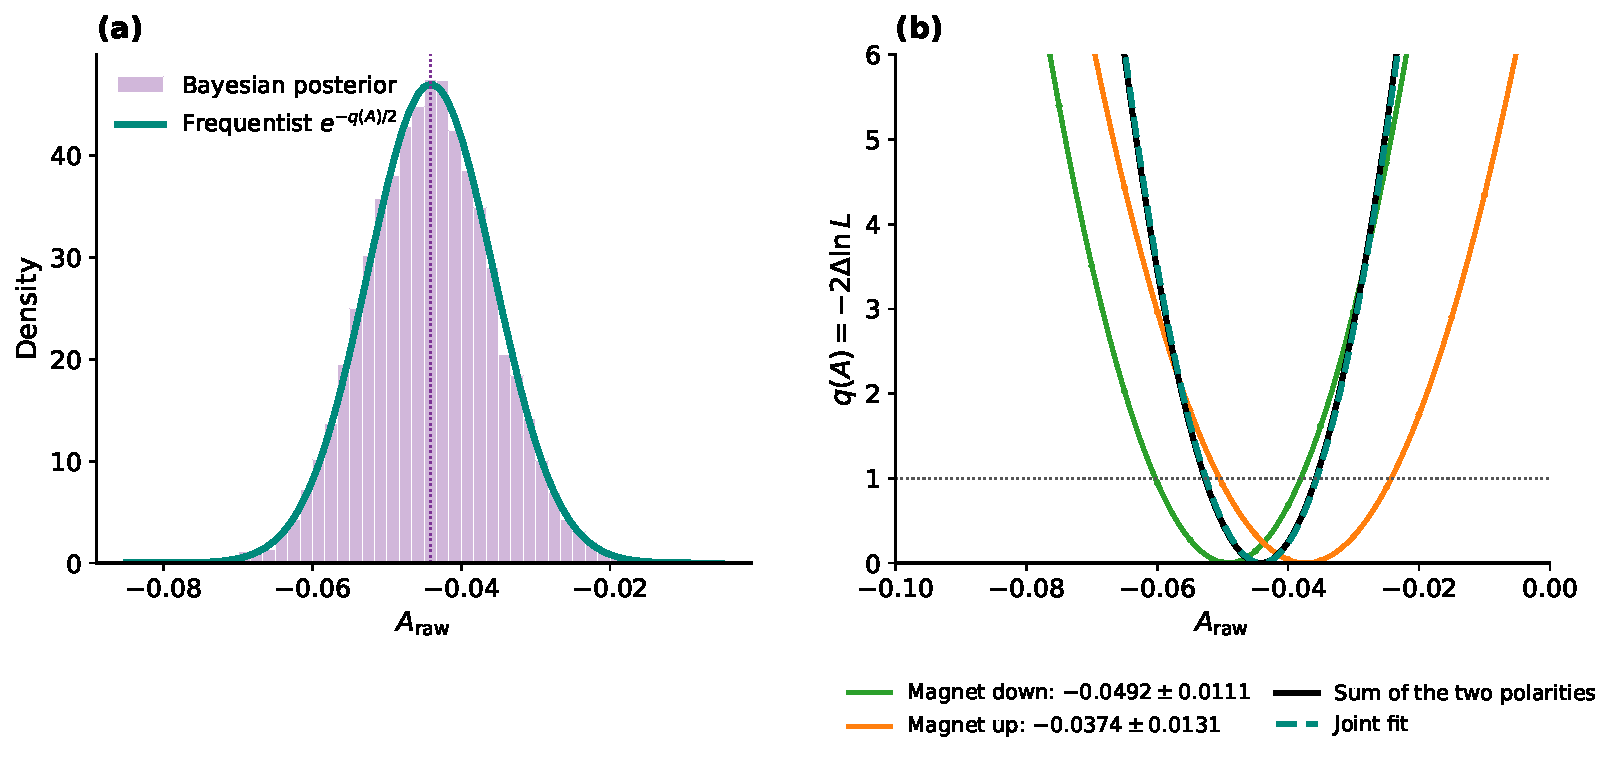
\includegraphics[width=0.95\textwidth]{figures/short_profile_polarity.pdf}
\caption{(a) Frequentist profile likelihood, $\exp[-q(A)/2]$ normalized, and Bayesian marginal posterior of $A$. (b) Profile curves $q(A)$ of the two magnet polarities (parabolic fits to the points), their sum and the joint fit.}
\label{fig:checks_profile}
\end{figure*}

\emph{Hypothesis test.} Three tests of $A=0$ are available. The exact binomial test of $N^-=N^+$ on all candidates gives $6.1\sigma$ ($A_{\mathrm{count}}=-0.0432\pm0.0071$); it sees signal and background together and does not use the mass. The Frequentist test of the fit gives $p=2\times10^{-7}$ ($Z=\sqrt{q(0)}=5.2\sigma$ in the two-sided convention, $5.06\sigma$ one-sided, Sec.~\ref{sec:appendix_freq}), independent of the prior and not the probability of $A=0$; its size and power were verified with toy MC (Sec.~\ref{sec:validation_power}).

The Bayes factor, $BF_{10}\approx9\times10^3$, depends on the prior width (Sec.~\ref{sec:bayes_factor}). For $A$ the Frequentist and Bayesian tests give the same conclusion; for the background asymmetry, $A_b=-0.040\pm0.018$, a Frequentist test would call $2.3\sigma$ a hint while $BF_{01}\approx3.5$ mildly favors $A_b=0$: the $p$-value asks how improbable the data are under $A_b=0$, the Bayes factor which hypothesis the data prefer after the prior volume is accounted for.

\subsection{Comparison with the Published Analysis}
\label{sec:comparison_published}
\emph{In short: the published value ($-0.060\pm0.007$) differs from this one ($-0.0441\pm0.0085$) by the sample and the model; with the same $D^0$ veto the Bayesian fit gives $-0.0496\pm0.0088$, and $\Araw$ is not $\ACP$.}
The published analysis~\cite{lhcb_cpv_2013} finds $\Araw=-0.060\pm0.007$ with $22{,}119\pm164$ signal candidates, against $-0.0441\pm0.0085$ and $15{,}328\pm133$ here: the Open Data record is a preselected subset and the published model has a Cruijff signal, partially reconstructed four-body decays and a misidentified peaking background from simulation. With the same $D^0$ veto the Bayesian fit gives $-0.0496\pm0.0088$, within $0.93\sigma$ of the published value.

The raw asymmetry is not the CP asymmetry: $\ACP\approx\Araw-A_P-A_D$ (Eq.~\eqref{eq:acp}), and in the published analysis the corrections move the result from $-0.060$ to $-0.043\pm0.009\pm0.003\pm0.007$ ($3.7\sigma$)~\cite{lhcb_cpv_2013}, by $+0.017$, about two statistical uncertainties of this work. Such a correction cannot be assumed for a different selection, and the $5.2\sigma$ here is the significance of a nonzero raw asymmetry, not of CP violation. A later measurement on a larger data set gives $\ACP=-0.037\pm0.002\pm0.002\pm0.003$ ($8.5\sigma$)~\cite{lhcb_cpv_prd2023,lhcb_cpv_paper}; our result is consistent with these in sign and size.

\subsection{Machine-Learning Cross-Check}
\label{sec:comparison_mlcheck}
\emph{In short: a classifier trained on weak labels from the mass spectrum selects candidates without changing $\Araw$ beyond its statistical spread; it does not improve the precision and cannot remove the misidentified decays under the signal (Sec.~\ref{sec:ml}).}
A cut at $0.5$ on the classifier score keeps $92\%$ of the fitted signal and $36\%$ of the background and gives $\Araw=-0.0451\pm0.0087$ (Bayesian) and $-0.0447\pm0.0086$ (Frequentist), against $-0.0443$ and $-0.0441$ for the full window: both shifts are within the statistical spread expected for a subsample (Sec.~\ref{sec:ml_stability}, Fig.~\ref{fig:ml_three}). The precision does not improve because the nominal sample has little background to remove; the classifier is described in Sec.~\ref{sec:ml}.


\subsection{Numerical Agreement}
\label{sec:comparison_numbers}
\emph{In short: the two fits agree to the quoted digits (estimates differ by $0.0002$, both uncertainties are $0.0085$, systematic uncertainties $0.0070$ and $0.0072$); sideband subtraction gives $-0.0503\pm0.0083$.}
The two fits of the same model agree to the precision of the quoted digits: the estimates differ by $0.0002$ ($0.02$ standard deviations), the uncertainties are both $0.0085$, the $68\%$ and $95\%$ intervals differ by at most $0.0002$, and the shifts of the thirteen systematic variants agree within $0.0005$, with the same group uncertainties for the window ($0.0014$) and the preselection ($0.0058$) and slightly different ones for the background ($0.0037$ against $0.0040$) and the signal model ($0.0002$ against $0.0006$), so that the total systematic uncertainties are $0.0070$ and $0.0072$ (Sec.~\ref{sec:syst}). A third estimate, by sideband subtraction (counting in the signal region after removing the background expected from the sideband fit), gives $-0.0503\pm0.0083$, which differs from the nominal value by $0.006$, less than one standard deviation, on the same candidates. This is expected, and it is not by itself a validation of the model. With $\sim2\times10^4$ candidates and flat priors the posterior is proportional to the likelihood, the likelihood is close to a Gaussian in $A$, and the posterior mode coincides with the maximum-likelihood estimate; the posterior median, the posterior mean and the mode differ by less than $2\times10^{-4}$. What the agreement does show is that neither the sampling (MCMC) nor the asymptotic approximations (Hesse, Wilks) introduce a bias: the Bayesian intervals have the coverage of the Frequentist ones (Sec.~\ref{sec:bayes_toymc}) and the profile-likelihood interval has the coverage assumed by Wilks' theorem (Sec.~\ref{sec:freq_coverage}).

The agreement does not extend to the validity of the model itself. Both methods describe the same spectrum with the same Gaussian signal and double-exponential background, and neither reaches $\chi^2/\mathrm{ndof}\approx1$ (Sec.~\ref{sec:bayes_gof}); what protects $\Araw$ is that its value does not depend on the signal shape (shift $-0.0002$ with a Crystal Ball) and that the background treatment, the largest model dependence, is included in the systematic uncertainty.

\subsection{Profile Likelihood, Posterior and the Two Polarities}
\label{sec:checks_profile}
\emph{In short: profiling and marginalizing the nuisance parameters give the same distribution of $A$; the two magnet polarities agree with each other, and combining their likelihoods reproduces the joint fit.}
The Frequentist way of eliminating the nuisance parameters is to profile them, $q(A)=-2\Delta\ln L$ with the other parameters re-maximized at each $A$, the Bayesian one is to marginalize them; Fig.~\ref{fig:checks_profile}a shows that $\exp[-q(A)/2]$, normalized, and the marginal posterior coincide, as expected for a near-Gaussian likelihood and flat priors. The two polarities were fitted separately and their profile curves added, which is the combination of likelihoods of two independent measurements of the same parameter (Fig.~\ref{fig:checks_profile}b): magnet down gives $-0.0492\pm0.0111$, magnet up $-0.0374\pm0.0131$, their sum $-0.0443\pm0.0084$, against $-0.0441\pm0.0085$ of the joint fit (the nuisance parameters are shared in the joint fit, separate in the sum). The Bayesian counterpart is sequential: the posterior of magnet down used as the prior of magnet up gives $-0.0446\pm0.0086$ (Table~\ref{tab:checks_polarity}).


\begin{table}[h]
\centering
\resizebox{\ifdim\width>\linewidth\linewidth\else\width\fi}{!}{\begin{tabular}{lcc}
\toprule
 & Frequentist & Bayesian \\
\midrule
Magnet down & $-0.0492\pm0.0111$ & $-0.0497\pm0.0112$ \\
Magnet up & $-0.0374\pm0.0131$ & $-0.0378\pm0.0129$ \\
Combination of the two & $-0.0443\pm0.0084$ & $-0.0446\pm0.0086$ \\
Joint fit & $-0.0441\pm0.0085$ & $-0.0443\pm0.0085$ \\
\bottomrule
\end{tabular}}
\caption{$\Araw$ for the two magnet polarities and their combination, by the two methods; the Frequentist combination is the sum of the profile likelihoods of the two polarities, the Bayesian one the sequential update of the posterior.}
\label{tab:checks_polarity}
\end{table}

\subsection{Confidence and Credible Regions in $(A,A_b)$}
\label{sec:checks_region}
\emph{In short: the $68\%$ and $95\%$ regions of the Frequentist profile ($\Delta\mathrm{NLL}$ at the $\chi^2_2$ values $2.30$ and $5.99$) and of the Bayesian highest posterior density coincide, and $A=0$ lies outside both.}
For two parameters of interest the Wilks statistic follows a $\chi^2$ with two degrees of freedom (Fig.~\ref{fig:checks_region}). The background asymmetry is $A_b=-0.0402\pm0.0176$ (Hesse; Minos $[-0.0578,-0.0226]$), correlated with $A$ by $\rho=-0.16$ in the likelihood, $-0.17$ in the posterior, and $-0.17$ in the bootstrap. The point $A_b=0$ is at the edge of the $95\%$ region.

\begin{figure}[h]
\centering
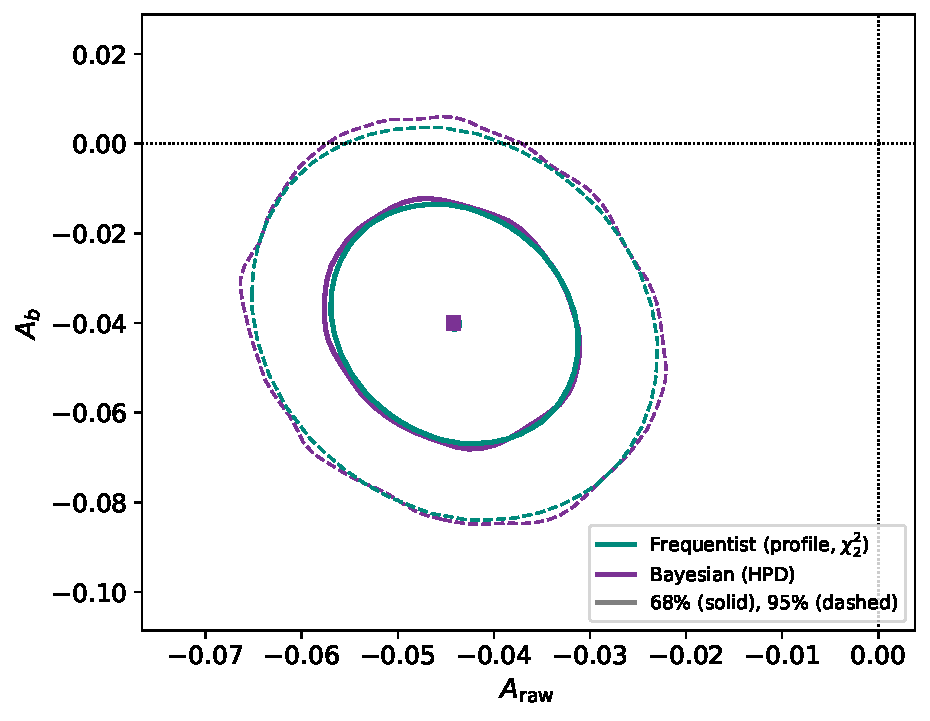
\includegraphics[width=\columnwidth]{figures/validation_region_Ab.pdf}
\caption{$68\%$ (solid) and $95\%$ (dashed) regions in $(A,A_b)$: Frequentist, from the profile likelihood with $\chi^2_2$ thresholds, and Bayesian, highest-posterior-density regions of the chain. Dots: best-fit and posterior median.}
\label{fig:checks_region}
\end{figure}

\subsection{Bayesian and Frequentist Intervals at Low Statistics}
\label{sec:bayes_lowstat}
\emph{In short: credible and confidence intervals coincide for $\sim2\times10^4$ candidates with flat priors, and stay equal, in value and coverage, down to $50$ candidates.}
With $\sim$$2\times10^4$ candidates the posterior is Gaussian and, with flat priors, the Bayesian and Frequentist results coincide by construction (Sec.~\ref{sec:bayes_posterior}). To find where they could differ, the same likelihood was analysed with both methods on toy-MC datasets of $N=50$, $150$, $500$ and $2000$ candidates, $300$ for each size. The model is the six-parameter one of Sec.~\ref{sec:bayes_minimal} (Gaussian signal, one exponential background shared by the charges), which stays identifiable down to a few tens of events; the parameters are those of its fit to the data, with the yields rescaled. Each replica is analysed with the MCMC (median and equal-tailed credible intervals) and by maximum likelihood with \texttt{iminuit} (Hesse intervals, and Minos intervals from the profile likelihood and Wilks' theorem).

\begin{figure*}[t]
\centering
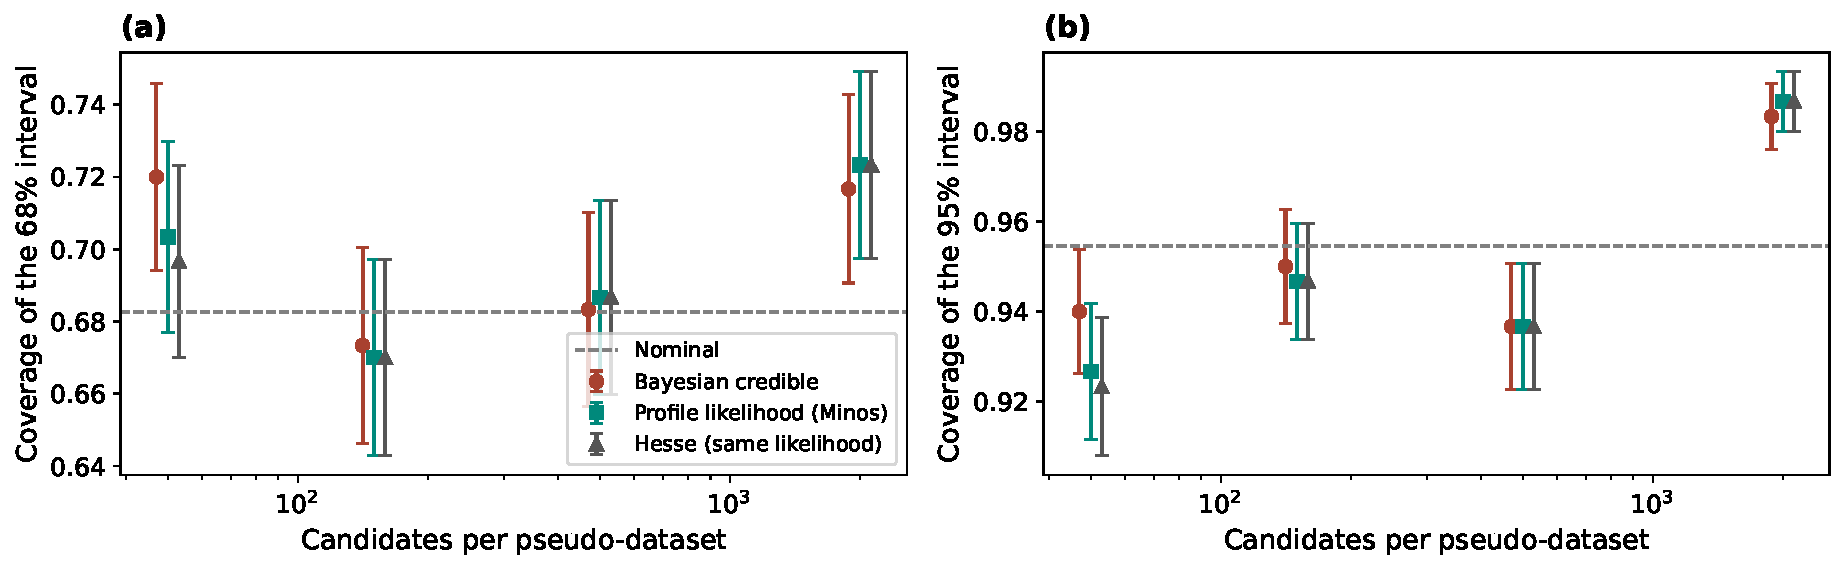
\includegraphics[width=0.95\textwidth]{figures/bayes_nominal_lowstat.pdf}
\caption{Coverage of the (a) 68\% and (b) 95\% intervals on $A$ vs the number of candidates, for the Bayesian credible interval, the profile-likelihood (Minos) interval and the Hesse interval of the same likelihood; 300 toy-MC datasets per point, binomial uncertainties. The dashed lines mark the nominal coverage ($1\sigma$, $2\sigma$; the Bayesian 95\% interval is the 2.5--97.5\% one).}
\label{fig:bayes_lowstat}
\end{figure*}

The two methods agree at every size (Fig.~\ref{fig:bayes_lowstat}). The coverages of the three intervals are compatible with nominal and with each other, the posterior median and the maximum-likelihood estimate differ on average by $5\%$ of the statistical uncertainty at $N=50$ and by less above, and the credible intervals stay symmetric (at $N=50$ the shortest chain is only $\approx10$ autocorrelation times long, so the Monte Carlo error on the interval endpoints is larger there). The asymmetry is a ratio of Poisson yields, whose likelihood is close to Gaussian already with a few tens of signal events: in this problem flat-prior credible intervals and profile-likelihood confidence intervals give the same answer, and Wilks' theorem holds, down to $N=50$. The two approaches differ in what the interval means and in hypothesis testing (Sec.~\ref{sec:bayes_factor}), not in the numbers. At $N=2000$ all three intervals over-cover slightly ($0.98$--$0.99$ for the 95\% interval); since the effect is the same for the three methods, it is a feature of this set of replicas rather than of either inference.

\FloatBarrier
